\section{Descriptive Statistic}
\subsection{Distribution and Histograms}
\begin{figure}[H]
    \begin{center}
    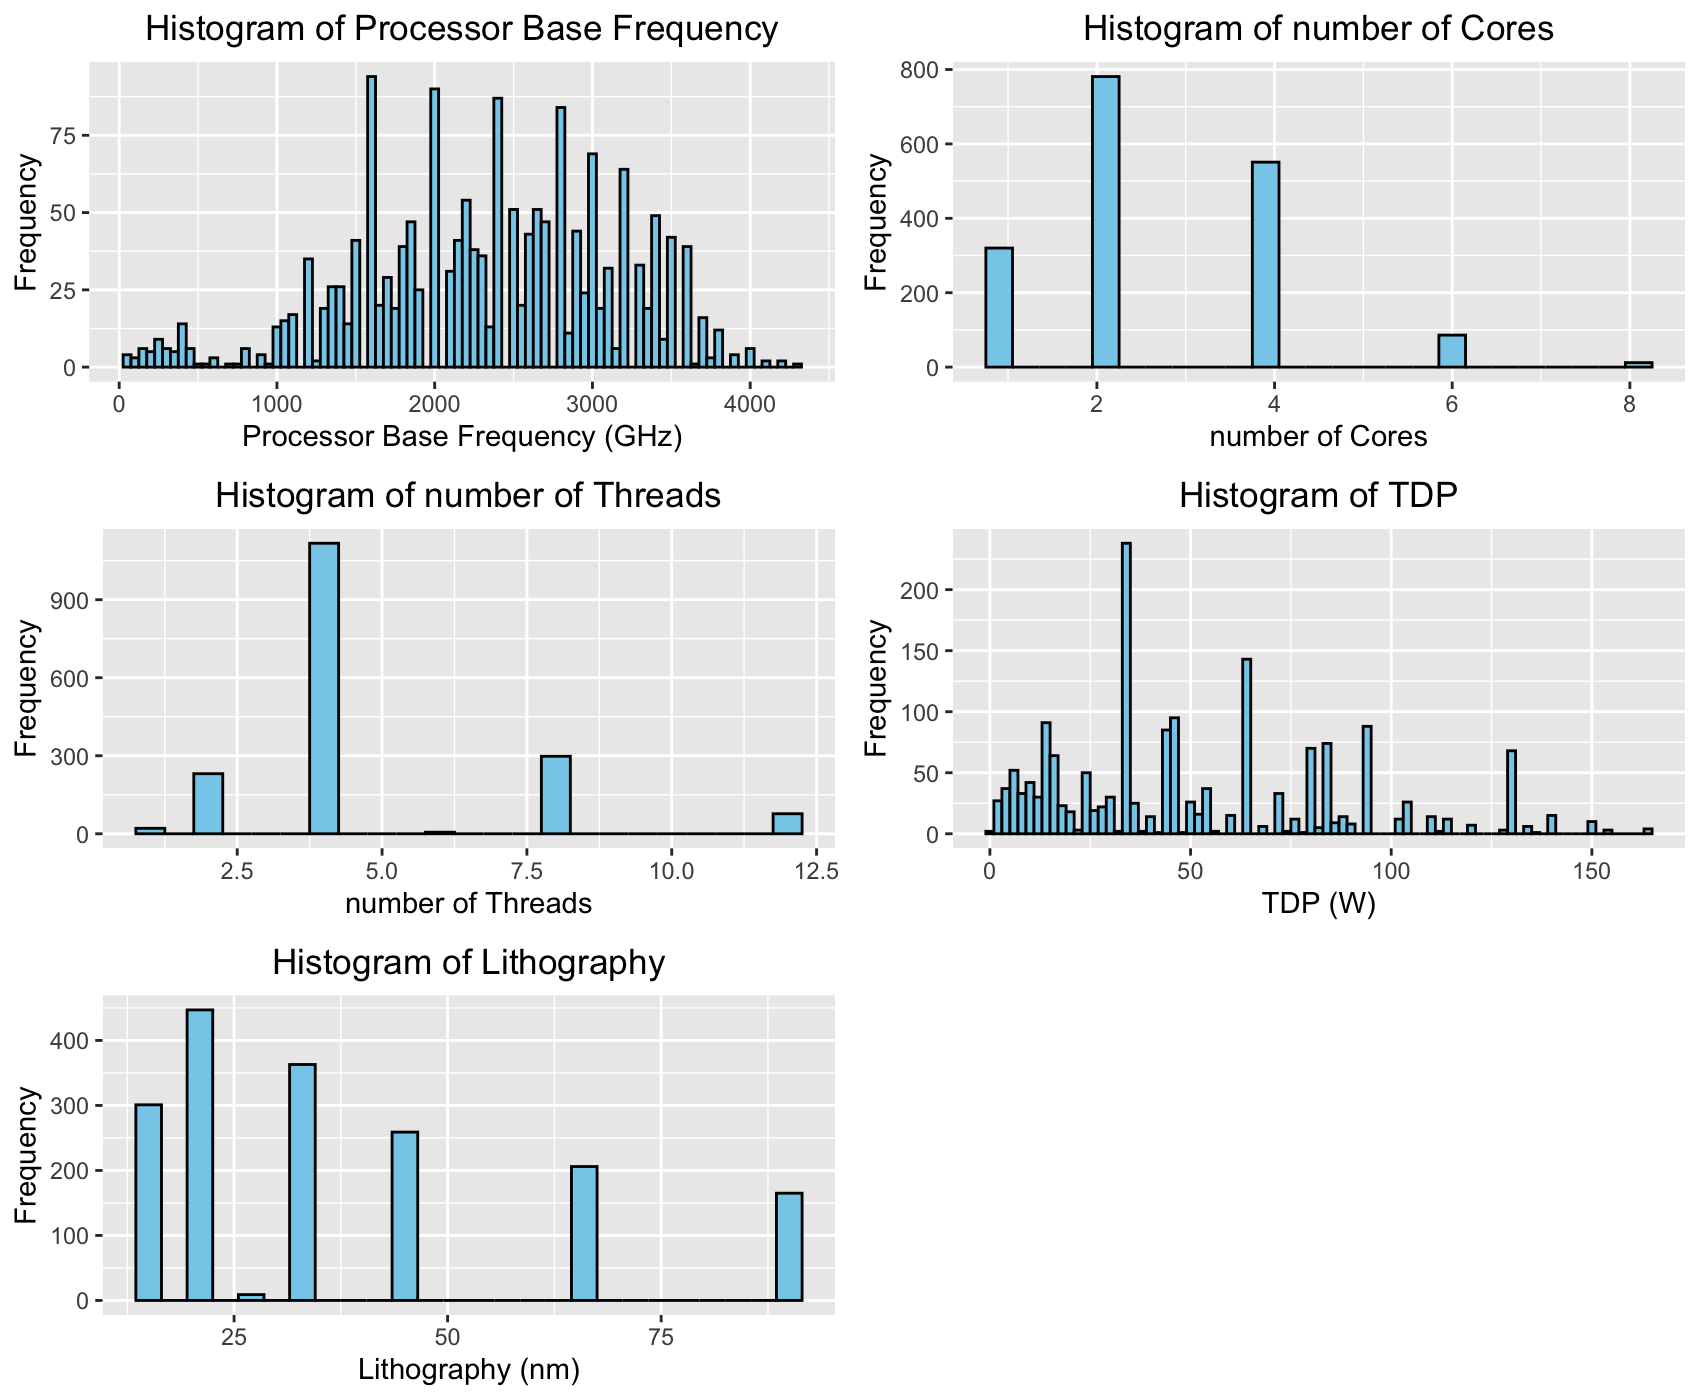
\includegraphics[width=14cm]{graphics/histogram.png}
    \end{center}
\end{figure}
\begin{itemize}
    \item Processor Base Frequency: 
    \begin{itemize}
        \item The frequencies range from 0 to around 4200 MHz, with most values concentrated between 1000 and 3500 MHz. 
        \item The distribution is relatively uniform within this range, with a slight peak around 2500 MHz.
    \end{itemize}
    
    \item Number of Cores: 
    \begin{itemize}
        \item The distribution of the number of cores is right-skewed.
        \item Most CPUs have 2 or 4 cores, with a significant peak at 2 cores. 
        \item There are fewer CPUs with 6 or 8 cores, indicating that higher core counts are less common in the dataset.
        \item This suggests that while multi-core processors are common, high-core-count CPUs are less frequent.        
    \end{itemize}

    \item Number of Threads: 
    \begin{itemize}
        \item Similar to the number of cores, the distribution of the number of threads is right-skewed.
        \item Most CPUs have either 4 or 8 threads, with a significant peak at 4 threads. 
        \item The dataset contains a smaller number of CPUs with other thread counts, such as 2, 6, and 12 threads.
        \item There are some CPUs with a significantly higher number of threads, indicating the presence of high-performance CPUs with technologies like Hyper-Threading.     
    \end{itemize}

    \item TDP (Thermal Design Power):
    \begin{itemize}
        \item TDP values range widely from 0 to 150 watts. There is a concentration of CPUs with TDP values around 50 watts, with several peaks in the distribution.
        \item There are a few CPUs with higher TDP values, which typically correspond to more powerful processors that require more cooling.
        \item This indicates that most CPUs are designed to operate within a standard thermal envelope, but high-performance CPUs demand more power.
    \end{itemize}

    \item Lithography: 
    \begin{itemize}
        \item The lithography histogram shows several peaks, indicating different manufacturing process nodes.
        \item Most CPUs have lithography sizes of either 14 nm or 22 nm, with significant peaks at these values. 
        \item Other common sizes include 32 nm and 45 nm, with fewer CPUs having lithography sizes of 10 nm or 7 nm.
        \item This reflects the advancements in semiconductor manufacturing technology, with newer CPUs being produced at smaller process nodes for improved performance and efficiency.
    \end{itemize}

\end{itemize}

Implications:
\begin{itemize}
    \item Processor Base Frequency: The relatively normal distribution suggests a common range of base frequencies, with few extreme values. This will influence our regression model, as we need to account for these outliers.

    \item Number of Cores and Threads: The right-skewed distributions indicate that while multi-core and multi-threading capabilities are common, the extent varies widely. High-core and high-thread CPUs, although fewer, represent the high-performance segment and should be carefully considered in our model.

    \item TDP: The distribution suggests that most CPUs are designed within certain power and thermal limits, but there are high-performance CPUs with higher TDP. This attribute is crucial as it impacts the CPU's ability to sustain higher clock speeds under load.

    \item Lithography: The presence of multiple peaks reflects the evolution of manufacturing processes over time. This attribute is essential for our model as newer process nodes typically allow for higher clock speeds and better efficiency.
\end{itemize}
By understanding these distributions, we can better prepare our data for inferential statistics and modeling, ensuring that our regression model accurately captures the relationship between these attributes and CPU clock speeds. This will involve handling outliers appropriately, scaling the features, and ensuring that the model is trained on a representative sample of the data.

\subsection{Boxplots for Outliers}
\begin{figure}[H]
    \begin{center}
    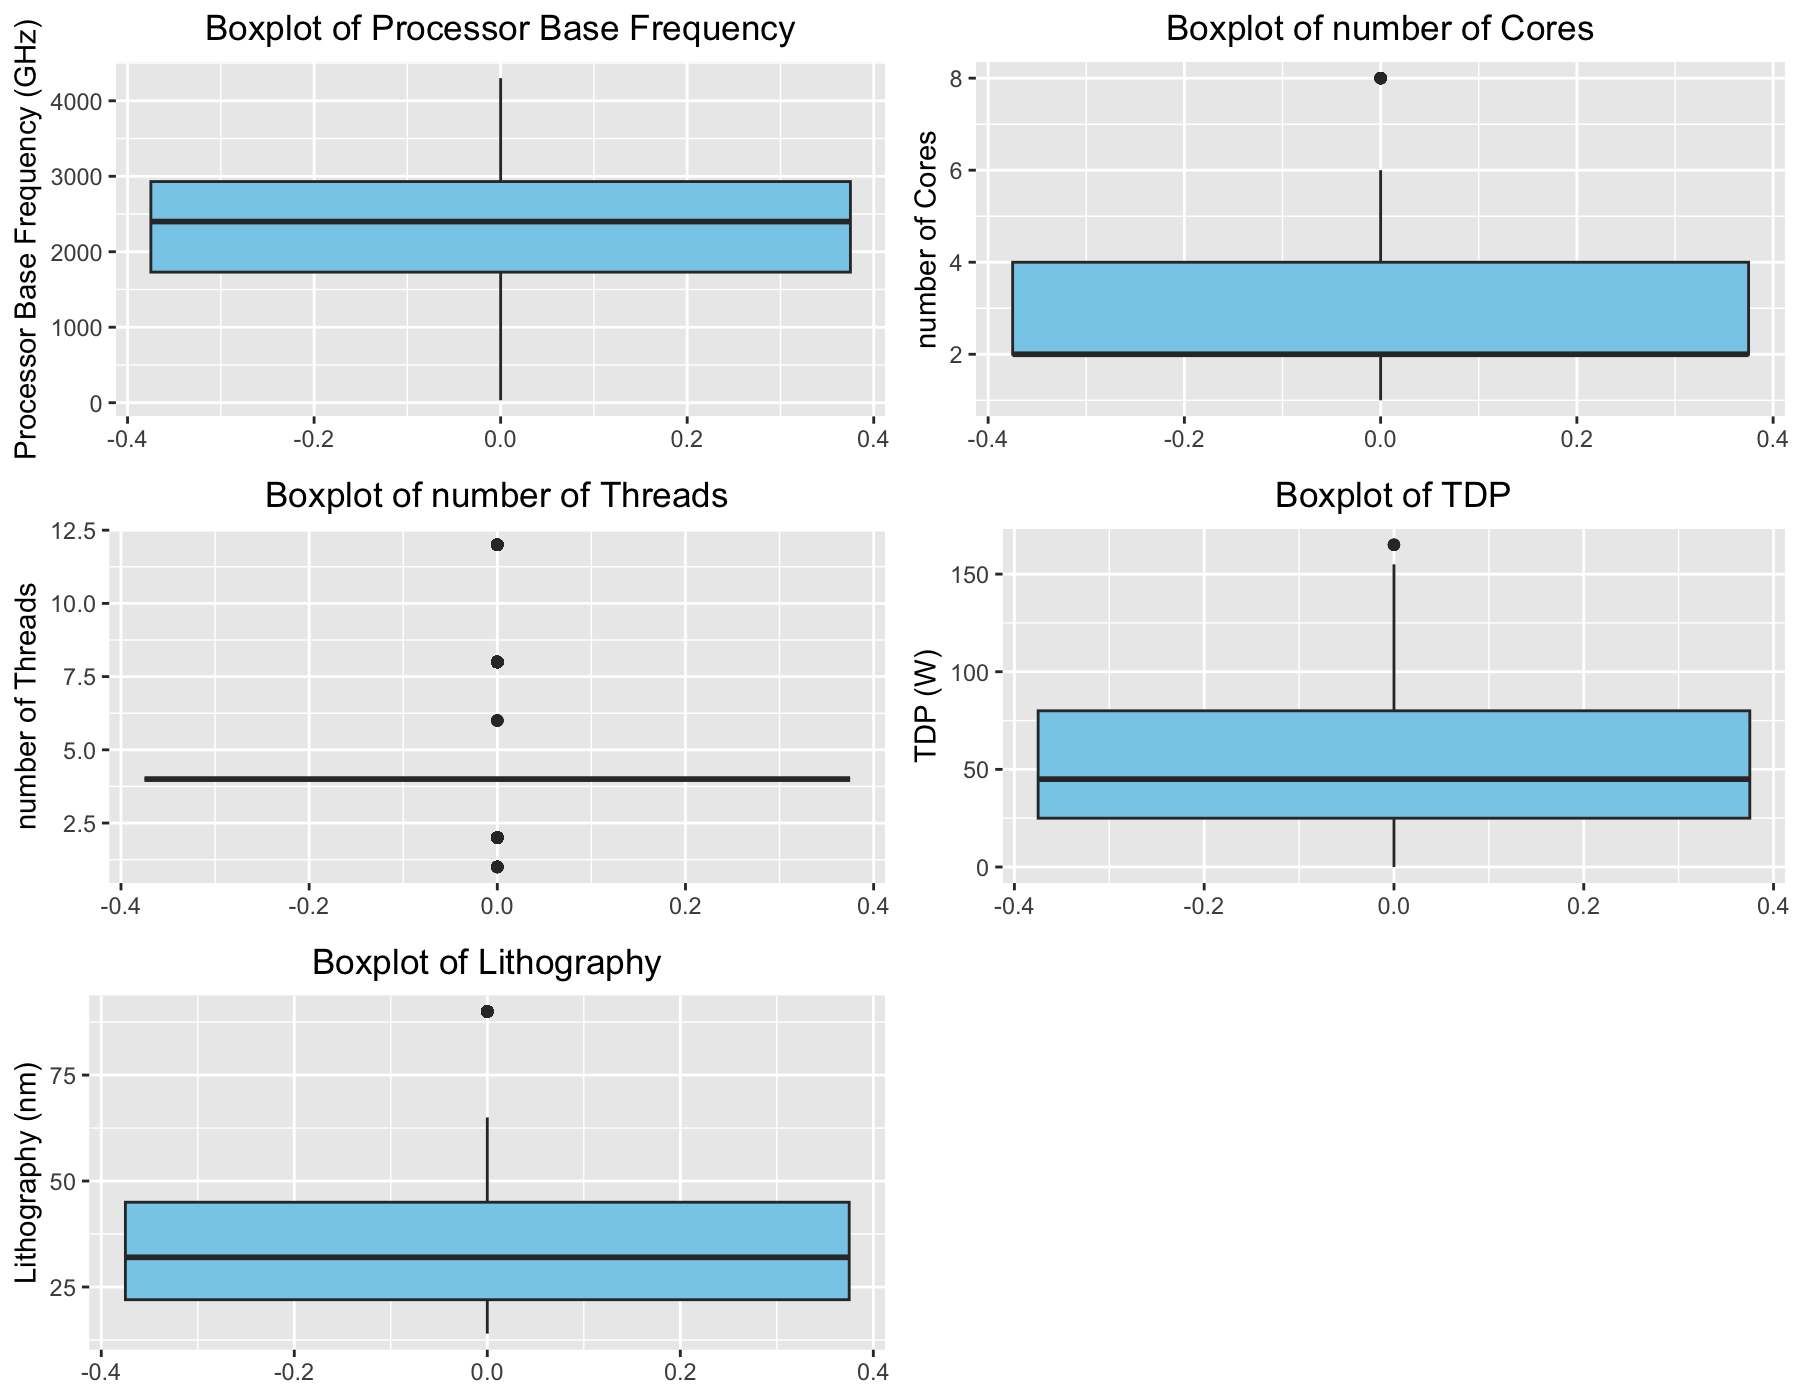
\includegraphics[width=14cm]{graphics/boxplot.png}
    \end{center}
\end{figure}
The boxplots provide a visual representation of the distribution, central tendency, and variability of key attributes in the dataset, as well as the presence of outliers. Here's a detailed explanation of each boxplot:

\begin{itemize}
    \item Boxplot of Processor Base Frequency (GHz):
    \begin{itemize}
        \item The median processor base frequency is around 2000 MHz. The interquartile range (IQR) spans from approximately 1000 to 3000 MHz. There are no significant outliers beyond this range, indicating a relatively symmetric distribution of base frequencies.
    \end{itemize}

    \item Boxplot of Number of Cores:
    \begin{itemize}
        \item The median number of cores is 2. The IQR ranges from 2 to 4 cores. There is one outlier at 8 cores, suggesting that while most CPUs have between 2 and 4 cores, there are a few models with a significantly higher core count.
    \end{itemize}

    \item Boxplot of Number of Threads:
    \begin{itemize}
        \item The median number of threads is 4. The IQR ranges from 4 to 8 threads. There are several outliers, both below 4 and above 8 threads, indicating that there are CPUs with unusual thread counts compared to the majority in the dataset.
    \end{itemize}
    
    \item Boxplot of TDP (W):
    \begin{itemize}
        \item The median TDP is around 50 watts. The IQR spans from approximately 30 to 75 watts. 
        \item There is one outlier above 150 watts, indicating that most CPUs have moderate power consumption, with a few exceptions having significantly higher TDP values.
    \end{itemize}

    \item Boxplot of Lithography (nm):
    \begin{itemize}
        \item The median lithography size is 22 nm. The IQR ranges from 22 to 32 nm. 
        \item There are a few outliers below 22 nm and one above 45 nm, indicating that while most CPUs have lithography sizes within this range, there are some with newer or older manufacturing technologies.
    \end{itemize}
\end{itemize}

Implications:
The boxplots provide several insights that are crucial for our project on predicting CPU clock speeds:

\begin{itemize}
    \item Processor Base Frequency:
    \begin{itemize}
        \item The central tendency and spread of base frequencies are important for understanding the typical performance range of CPUs in the dataset.
        \item The presence of outliers indicates that while most CPUs have base frequencies in a common range, some high-performance CPUs exist with higher base frequencies, which need to be considered in our model.
    \end{itemize}
    
    \item Number of Cores and Threads:
    \begin{itemize}
        \item The distributions show that multi-core and multi-threaded CPUs are common, but high-core and high-thread counts are less frequent, representing high-performance segments.
        \item Outliers in these attributes reflect high-performance CPUs, which can affect the overall performance trends and must be accurately modeled.
    \end{itemize}
    
    \item TDP:
    \begin{itemize}
        \item The central tendency and variability in TDP indicate the power and thermal characteristics of most CPUs.
        \item The outliers suggest that while most CPUs operate within a standard thermal range, some require much higher or lower power, influencing their ability to sustain higher clock speeds.
    \end{itemize}
    
    \item Lithography:
    \begin{itemize}
        \item The distribution of lithography values highlights the evolution of manufacturing technology, with most CPUs produced using advanced nodes like 22 nm and 32 nm.
        \item The outlier at few outliers below 22 nm and one above 45 nm represents older technology, which typically correlates with lower efficiency and performance.
    \end{itemize}
\end{itemize}
\subsection{Scatter plot for relationship between Processor Base Frequency with the others}
\begin{figure}[H]
    \begin{center}
    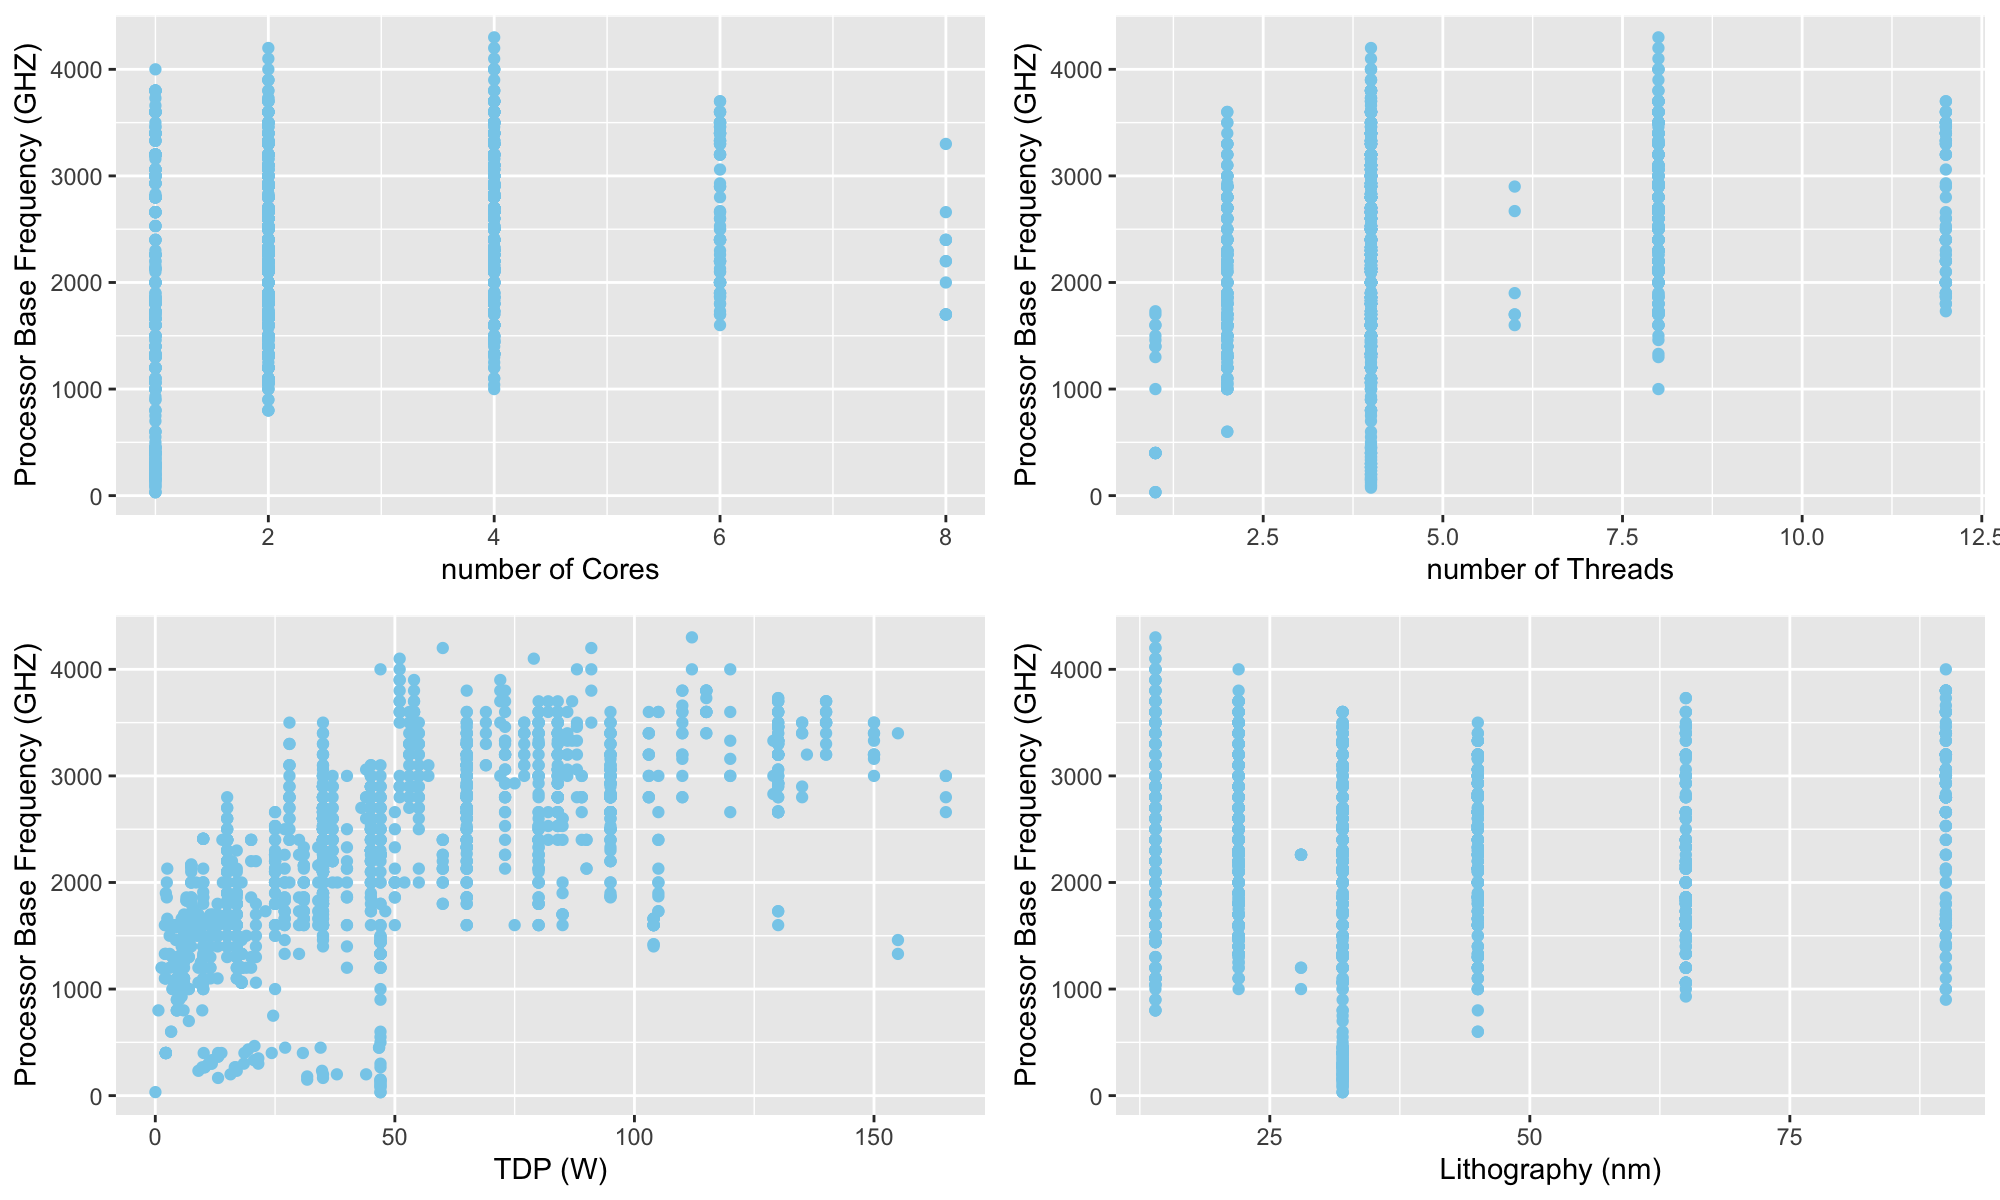
\includegraphics[width=14cm]{graphics/scatter.png}
    \end{center}
\end{figure}

\begin{itemize}
    \item Processor Base Frequency and Number of Cores
    \begin{itemize}
        \item The plot in the top left shows the relationship between the number of cores in a processor and its base frequency.
        \item The data points indicate an inverse relationship - as the number of cores increases, the processor's base frequency tends to decrease. This suggests that adding more cores may come at the cost of lower individual core frequencies.
    \end{itemize}

    \item Processor Base Frequency and Number of Threads
    \begin{itemize}
        \item The plot in the top right shows the relationship between the number of threads in a processor and its base frequency.
        \item The data points suggest a positive relationship - as the number of threads increases, the processor's base frequency generally increases as well. This implies that more threads can be supported without significantly impacting the core frequencies.
    \end{itemize}

    \item Processor Base Frequency and TDP
    \begin{itemize}
        \item The bottom left plot displays the relationship between the processor's Thermal Design Power (TDP) and its base frequency.
        \item The wide distribution of data points indicates that processor performance, as measured by base frequency, is not solely determined by power consumption (TDP). There are processors with a wide range of frequencies across various TDP values.
    \end{itemize}

    \item Processor Base Frequency and Lithography
    \begin{itemize}
        \item The bottom right plot illustrates the relationship between the processor's lithography (manufacturing process) and its base frequency.
        \item The data suggests that processors manufactured using smaller lithography sizes (in nanometers) tend to have higher base frequencies. This is likely due to the performance improvements enabled by advancements in semiconductor manufacturing technology.
    \end{itemize}
\end{itemize}
Overall, this set of scatter plots provides a comprehensive view of how different processor hardware specifications, such as core count, thread count, power consumption, and manufacturing process, are related to the fundamental performance metric of processor base frequency.

\subsection{Correlation Matrix}
\begin{figure}[H]
    \begin{center}
    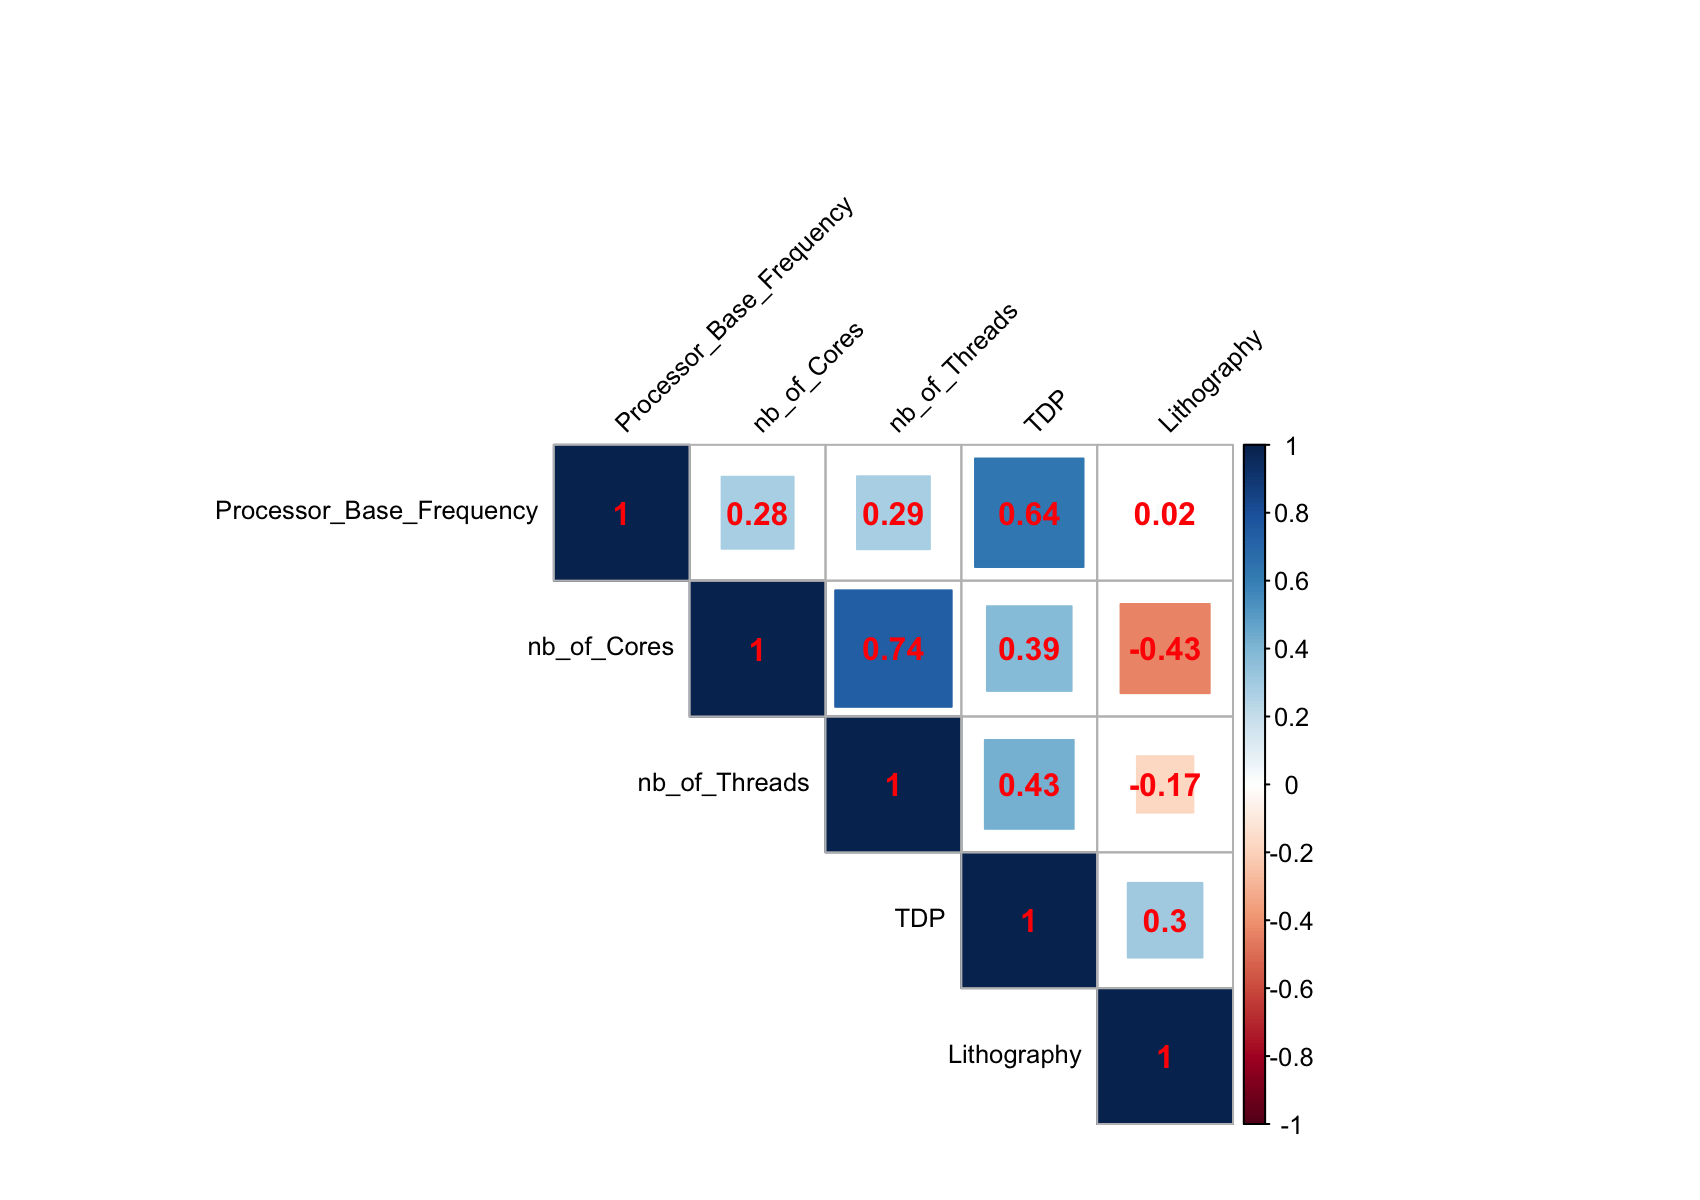
\includegraphics[width=14cm]{graphics/correlation_matrix.png}
    \end{center}
\end{figure}

The correlation matrix provides a comprehensive view of the linear relationships between pairs of variables in our dataset. Each cell in the matrix represents the correlation coefficient between two variables, ranging from -1 (perfect negative correlation) to 1 (perfect positive correlation). Here's a detailed explanation of the matrix for our project:\\[6pt]
Key Observations:
\begin{itemize}
    \item Processor Base Frequency:
    \begin{itemize}
        \item Correlation with TDP: The strongest positive correlation is with TDP (0.64). This indicates that CPUs with higher base frequencies generally have higher thermal design power requirements. This is expected as higher clock speeds typically result in greater power consumption and heat generation.
        \item Negative Correlation with Lithography: There is a moderate negative correlation with Lithography (0.02). This suggests that CPUs manufactured with smaller process nodes tend to have higher base frequencies. Advanced manufacturing technologies often result in better performance characteristics.
    \end{itemize}
    
    \item Number of Cores:
    \begin{itemize}
        \item Strong Positive Correlation with Number of Threads (0.74): This high correlation is expected as CPUs with more cores generally support more threads, especially with technologies like Hyper-Threading.
        \item Negative Correlation with Lithography (-0.43): Indicates that CPUs with a higher number of cores tend to be manufactured using smaller lithography nodes, aligning with advancements in CPU design that pack more cores into smaller spaces.
    \end{itemize}
    
    \item Number of Threads:
    \begin{itemize}
        \item Positive Correlation with TDP (0.43): Similar to the base frequency, a higher number of threads is associated with higher TDP, reflecting increased power consumption and heat dissipation needs.
    \end{itemize}
    
    \item TDP:
    \begin{itemize}
        \item Slight Positive Correlation with Lithography (0.3): This weak correlation suggests that the thermal design power does not have a strong relationship with the manufacturing process node.
    \end{itemize}
    
    \item Lithography:
    \begin{itemize}
        \item Negative Correlations with Other Variables: Lithography shows a general negative correlation with performance-related attributes, reinforcing the trend that smaller manufacturing nodes (indicative of newer technologies) are associated with higher performance capabilities.
    \end{itemize}
\end{itemize}

Implications:
\begin{itemize}
    \item The correlation matrix is crucial for understanding the relationships between different CPU attributes and their collective impact on clock speed. Here are some key takeaways for our project on predicting CPU clock speeds:
    
    \item TDP and Processor Base Frequency: The strong positive correlation suggests that models predicting clock speed should account for TDP as a significant predictor.
    
    \item Manufacturing Process (Lithography): The negative correlations with performance attributes highlight the importance of considering lithography advancements in performance modeling.
    
    \item Number of Cores and Threads: The strong inter-correlation indicates that either variable could be used interchangeably in some modeling contexts, but including both provides a more nuanced understanding of CPU capabilities.
\end{itemize}


\newpage
